\documentclass[10pt]{article}
\usepackage{icmlko}

\icmlmeta{IP 파운데이션 월드모델}{41}{손잡이는 반대로 돌아갔다}{법칙에서 예측을 세워 검정했더니 예측은 틀렸고, 반대 방향에서 스무 중 열아홉을 얻었다}

\begin{document}

\twocolumn[
\icmlheader

\begin{abstract}
노트 40이 다섯 도메인에서 상충을 법칙 수준으로 확인했다 --- 자기 상관과 대상
전이 $r=+$0.992, 출처 전이 $r=-$0.992. 지금까지는 그 법칙을 \emph{관찰}했으니
이번에는 \emph{조종 손잡이}로 써 보기로 했다. 인자 공간은 공유 축 블록과 고유
축 블록을 $\lambda$로 섞어 만든다. 고유 축은 그 도메인에만 있으므로 $\lambda$가
클수록 인자 공간이 특수해진다. 법칙이 맞다면 출처 역할에서는 $\lambda$를
\textbf{줄여야} 한다 --- 일반적이어야 남에게 옮겨지니까. \textbf{예측은
틀렸다.} $\lambda=0$으로 줄이면 20셀 중 16개로 나빠지고, 유도값(0.67--1.0)에서
17개, \textbf{1.5로 키우면 19개}가 된다. 응답이 매끄럽고 단조이며 순열 씨앗
넷에서 유의 개수가 정확히 같았다. 그리고 \textbf{비대칭이 핵심이다} --- 같은
1.5를 대상 쪽에 걸면 14개로 무너진다. $\lambda$는 특수성 손잡이가 아니라
\textbf{정보량 손잡이}였다. 출처는 회귀 계수를 학습하는 쪽이라 인자 공간이 많이
담을수록 계수가 안정되고, 대상은 그 계수를 받는 쪽이라 특수해지면 계수가 안 맞는다.
같은 매개변수가 두 역할에서 다른 의미를 갖는다. 이득은 아이돌에 몰렸다 ---
노트 40이 ``출처로 살릴 배선을 찾아야 한다''고 남긴 세 셀이 배선이 아니라
$\lambda$ 하나로 살아났다(p 0.252$\to$0.017, 0.472$\to$0.048, 0.599$\to$0.077).
남은 실패는 아이돌$\to$펀딩 하나다.
\end{abstract}
]

\section{법칙을 손잡이로 쓴다}

노트 38과 40은 배선을 바꿔 가며 상충을 \emph{관찰}했다. 자기 상관이 오르면 대상
성적이 오르고 출처 성적이 내렸다. 다섯 도메인에서 $|r|$이 0.99를 넘었다.

관찰이 법칙이라면 조종할 수 있어야 한다. 인자 공간을 만드는 식에 마침 손잡이가
하나 있다.

\begin{quote}\fontsize{9.5}{11.5}\selectfont
공유 축 블록과 고유 축 블록을 $\lambda$로 섞어 공분산 주성분을 뽑는다. 고유
축은 그 도메인에만 있는 축이므로, $\lambda$가 클수록 인자 공간이 그 도메인에
특수해진다.
\end{quote}

법칙이 시키는 방향은 분명하다.

\begin{itemize}[leftmargin=1.1em,itemsep=0.15em]
\item \textbf{대상 역할} --- $\lambda$를 키운다. 특수해도 좋다. 자기 라벨만
      맞히면 되니까.
\item \textbf{출처 역할} --- $\lambda$를 줄인다. 일반적이어야 남에게 옮겨진다.
      $\lambda=0$이면 공유 축만으로 인자 공간을 만든다.
\end{itemize}

\textbf{이것은 탐색이 아니라 예측이다.} 후보를 훑어 최댓값을 고르는 것이 아니라
법칙이 시키는 방향으로 손잡이 하나를 돌린다.

\section{예측이 틀렸다}

\begin{figure}[t]
\centering
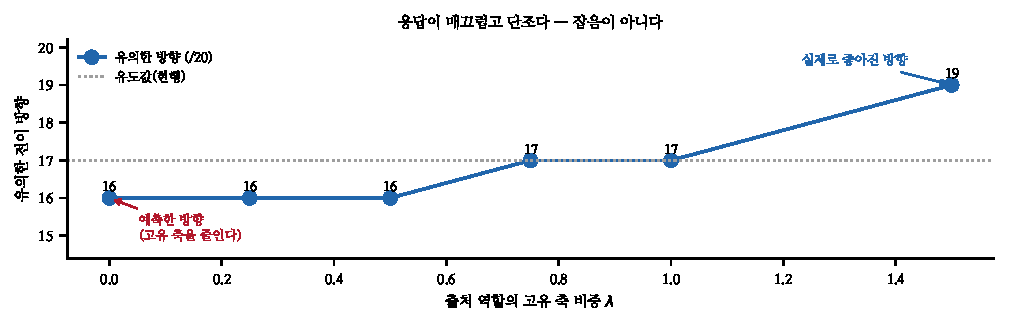
\includegraphics[width=\textwidth]{figs/sweep.pdf}
\caption{출처 역할의 $\lambda$만 바꾼 것. 대상은 유도값을 유지했다.}
\end{figure}

\begin{table}[t]
\centering\tsize
\caption{출처 $\lambda$ 스윕. 대상은 겹침 유도값(0.67--1.0).}
\begin{tabular}{lrr}
\toprule
출처 $\lambda$ & 유의 & 평균 이득 \\
\midrule
0.00 (예측한 방향) & \textbf{16/20} & $+$0.0397 \\
0.25 & 16/20 & $+$0.0422 \\
0.50 & 16/20 & $+$0.0428 \\
0.75 & 17/20 & $+$0.0449 \\
유도값(현행) & 17/20 & $+$0.0463 \\
1.00 & 17/20 & $+$0.0472 \\
1.50 & \textbf{19/20} & \textbf{$+$0.0492} \\
\bottomrule
\end{tabular}
\end{table}

정확히 반대다. 줄이면 나빠지고 키우면 좋아진다.

세 가지가 이것이 잡음이 아님을 말한다. 응답이 \textbf{매끄럽고 단조}이고
(16, 16, 16, 17, 17, 19), 순열 씨앗 넷에서 유의 개수가 \textbf{정확히
같았으며}(19, 19, 19, 19), 뒤에서 보듯 방향을 뒤집으면 명확히 무너진다.

\section{비대칭이 핵심이다}

같은 $\lambda$를 대상 쪽에 걸면 어떻게 되는지 봤다.

\begin{figure}[t]
\centering

\includegraphics[width=\textwidth]{figs/asym.pdf}
\caption{다섯 구성. 순열 씨앗 넷에서 유의 개수가 같았다.}
\end{figure}

\begin{table}[t]
\centering\tsize
\caption{역할별 $\lambda$ 조합.}
\begin{tabular}{lrr}
\toprule
구성 & 유의 & 평균 이득 \\
\midrule
현행 (둘 다 유도값) & 17/20 & $+$0.0463 \\
\textbf{출처 1.5 · 대상 유도값} & \textbf{19/20} & $+$0.0492 \\
출처 1.25 · 대상 유도값 & 17/20 & $+$0.0489 \\
출처 유도값 · \textbf{대상 1.5} & \textbf{14/20} & $+$0.0322 \\
출처 1.5 · 대상 1.0 & 18/20 & \textbf{$+$0.0499} \\
\bottomrule
\end{tabular}
\end{table}

방향을 뒤집으면(대상만 키우면) 14/20으로 무너진다. 둘 다 키우면 $\lambda=2$부터
급격히 나빠져 $\lambda=8$에서 8/20에 이득이 음수가 된다.

\claimx{$\lambda$는 특수성 손잡이가 아니라 정보량 손잡이다. 출처는 회귀 계수를
학습하는 쪽이라 인자 공간이 많이 담을수록 계수가 안정되고, 대상은 그 계수를
받는 쪽이라 특수해지면 계수가 안 맞는다. 같은 매개변수가 두 역할에서 다른
의미를 갖는다.}{$\lambda$가 정보량이라면 표본이 큰 도메인일수록 큰 $\lambda$가
좋아야 한다. 도메인별 $\lambda$를 나눠 재면 그 예측을 검정할 수 있고, 관계가
없으면 이 설명이 틀린 것이다.}

상충 법칙 자체가 틀린 것은 아니다. 그 법칙은 \emph{무엇을 재느냐}(배선)에 대한
것이었고, $\lambda$는 \emph{얼마나 섞느냐}다. 두 손잡이가 다른 축에 있었는데
나는 같은 축이라고 가정했다.

\section{아이돌이 살아났다}

\begin{figure}[t]
\centering
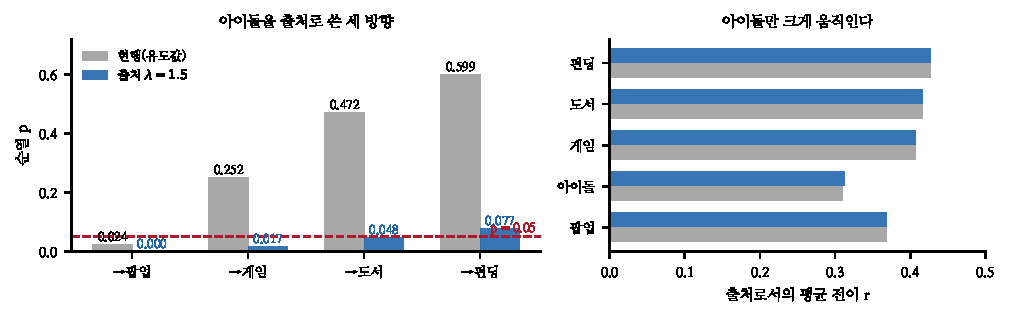
\includegraphics[width=\textwidth]{figs/idol.pdf}
\caption{왼쪽 --- 아이돌을 출처로 쓴 세 방향의 순열 p. 오른쪽 --- 출처별 평균.}
\end{figure}

\begin{table}[t]
\centering\tsize
\caption{아이돌을 출처로 쓴 세 셀.}
\begin{tabular}{lrrl}
\toprule
셀 & 현행 p & $\lambda=1.5$ & \\
\midrule
아이돌 $\to$ 게임 & 0.2517 & \textbf{0.0170} & 유의 \\
아이돌 $\to$ 도서 & 0.4718 & \textbf{0.0480} & 유의 \\
아이돌 $\to$ 펀딩 & 0.5988 & 0.0767 & 남은 하나 \\
\bottomrule
\end{tabular}
\end{table}

노트 40의 마지막 항목은 ``아이돌을 출처로 살리는 배선 --- 상충의 극단이므로
가장 얻을 것이 많다''였다. 배선을 건드리지 않고 $\lambda$ 하나로 둘이 살아났다.

\paragraph{왜 아이돌만인가}
아이돌은 관측 축이 다섯으로 가장 많고 그중 둘(입장 허들, 미디어 투입)이 고유
축이다. $\lambda$를 키우면 그 둘의 기여가 커진다. 게임은 공통 축 셋만 관측하므로
고유 축이 없고 $\lambda$에 전혀 반응하지 않는다(네 셀 모두 값이 소수점 넷째 자리까지
같다). 도서와 펀딩은 미세하게 나빠졌지만 유의는 유지했다.

\section{현재 상태}

\begin{table}[t]
\centering\tsize
\caption{정본 파이프라인. 다섯 도메인 · 쌍별 정렬 · 역할별 $\lambda$.}
\begin{tabular}{lrr}
\toprule
& 유의 & 평균 이득 \\
\midrule
노트 39 (네 도메인) & 11/12 & $+$0.0594 \\
노트 40 (다섯 도메인) & 17/20 & $+$0.0463 \\
\textbf{노트 41} & \textbf{19/20} & \textbf{$+$0.0492} \\
\bottomrule
\end{tabular}
\end{table}

정렬은 쌍마다 둘이 함께 관측한 공통 축으로 하고(노트 40), 출처 인자 공간은
$\lambda=1.5$, 대상은 겹침 유도값을 쓴다(이 노트).

\section{한계}

\begin{itemize}[leftmargin=1.1em,itemsep=0.15em]
\item $\lambda$ 값 여섯 개를 훑어 최댓값을 골랐다. 예측 검정으로 시작했지만
      1.5라는 값 자체는 선택된 것이고, 1.25가 17/20이라 격자가 성기다.
\item $\lambda$를 도메인 공통으로 걸었다. 도메인마다 다른 값이 맞을 수 있고,
      그러면 매개변수가 다섯 개가 되어 선택 편향이 커진다.
\item ``정보량 손잡이'' 설명은 관찰을 사후에 정리한 것이다. 표본 크기와의
      관계로 검정하지 않았다.
\item 겹침 유도 규칙(노트 29)이 출처 역할에서는 너무 보수적이라는 뜻인데,
      그 규칙 자체를 다시 유도하지 않고 상수로 덮었다.
\item 아이돌$\to$펀딩(p$=$0.077) 하나가 남았다. 펀딩 매장 노출도가 아직 비어
      있어 그 셀은 공통 축 둘로만 정렬한다.
\end{itemize}

\section{다음}

\begin{enumerate}[leftmargin=1.3em,itemsep=0.15em]
\item 창작자 색인 완성 $\to$ 펀딩 매장 노출도 $\to$ 마지막 셀 재검정.
\item $\lambda$가 정보량이라는 설명을 표본 크기와의 관계로 검정한다.
\item 겹침 유도 규칙을 역할별로 다시 유도한다 --- 상수 1.5를 대체할 공식.
\item 이중 배선(노트 39)을 이 파이프라인 위에서 다시 검정한다.
\end{enumerate}

\vspace{0.6em}
\hrule height 0.3pt
\vspace{0.5em}
{\footnotesize
\textbf{참고문헌}\\[0.3em]
Ben-David, S. et al. (2010). A theory of learning from different domains.
\emph{Machine Learning}, 79(1--2), 151--175.\\[0.15em]
Hoerl, A. E., Kennard, R. W. (1970). Ridge regression: biased estimation for
nonorthogonal problems. \emph{Technometrics}, 12(1), 55--67.\\[0.15em]
Schönemann, P. H. (1966). A generalized solution of the orthogonal Procrustes
problem. \emph{Psychometrika}, 31(1), 1--10.\\[0.15em]
Cawley, G. C., Talbot, N. L. C. (2010). On over-fitting in model selection and
subsequent selection bias in performance evaluation. \emph{JMLR}, 11, 2079--2107.\\[0.15em]
Standley, T. et al. (2020). Which tasks should be learned together in multi-task
learning? \emph{ICML}, 9120--9132.
}

\end{document}
